\documentclass[12pt]{article}
\usepackage[francais]{babel}
\usepackage[utf8]{inputenc}
\usepackage[T1]{fontenc}
\usepackage{graphicx}
\usepackage{fancyhdr}
\usepackage{hyperref}
\usepackage{float}
\usepackage{amsmath}
\usepackage[margin=1in]{geometry}
\usepackage{indentfirst}
\usepackage{titlesec}
\usepackage{appendix} 
\newcommand{\sectionbreak}{\clearpage}

\setlength{\parindent}{0cm}
%presentation of the document
\title{Projet Modélisation et Programmation Orientée Objet\smallbreak Documentation utilisateur\smallbreak Quatrième année - Informatique }
\author{Alexandre \textsc{Audinot},  Dan \textsc{Seeruttun-{}-Marie}}
\date{16/01/2015}
\begin{document}
\maketitle

\begin{figure}[!h] 
\centerline{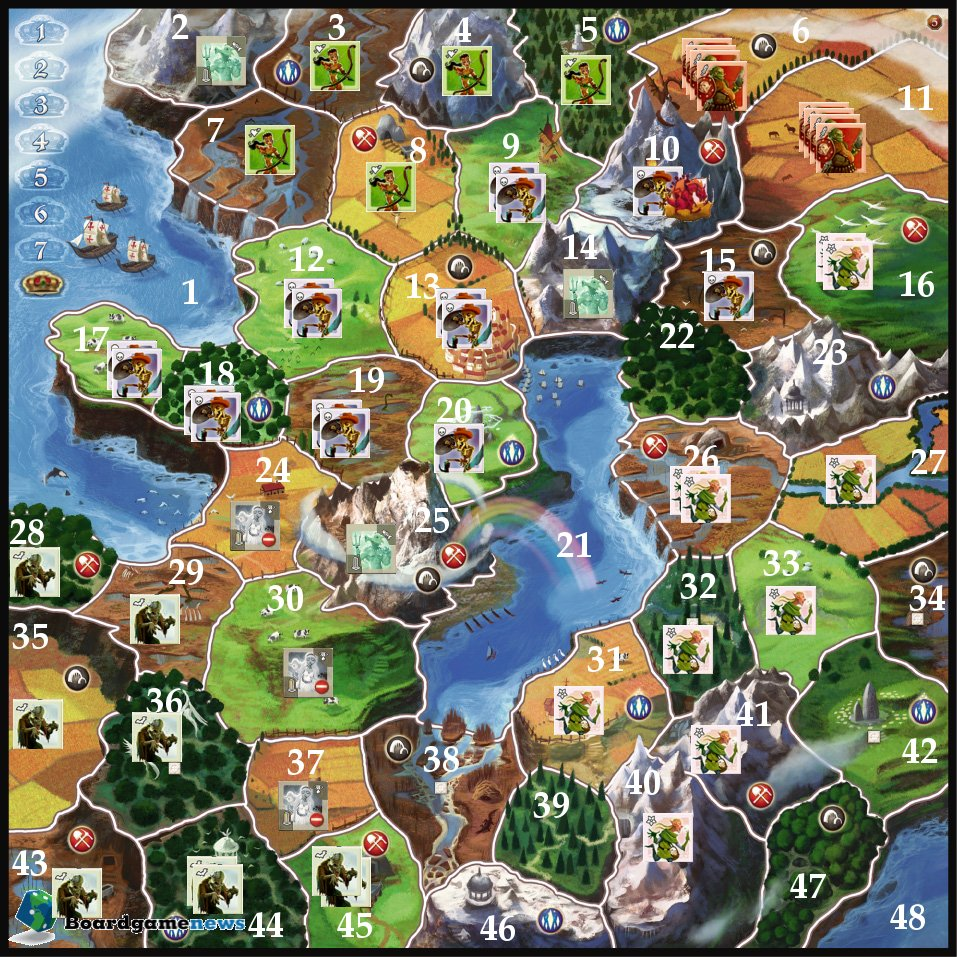
\includegraphics[scale=0.30]{img/cover.jpg}}
\end{figure}
\newpage

\newpage
%to add a table of contents
\tableofcontents
\newpage

\section{Principes du jeu}
\input{"principes.tex"}
\newpage
\section{Le jeu}
\input{"jeu.tex"}
\end{document}


